\section{Symmediane}\label{kapitel:Symmediane}
In diesem Kapitel werden wir zwei schwere Geometrieaufgaben besprechen. Wie üblich findet ihr am Ende des Kapitels Tipps und danach Lösungen zu beiden Aufgaben. Angesichts der Schwierigkeit ist es keine Schande, wenn ihr die Tipps verwendet oder euch die Lösungen durchlest.
\begin{aufgabe*}[**]\label{aufgabe:MEMO2014}
	Sei $ABC$ ein Dreieck und sei $D$ der Berührpunkt des Inkreises $\omega$ mit der Seite $\overline{BC}$. Sei $I_a$ der Mittelpunkt des Ankreises gegenüber $A$ und sei $L$ der von $D$ verschiedene Schnittpunkt von $AD$ mit $\omega$. Schließlich sei $M$ der Mittelpunkt von $\overline{BC}$ und $N$ der Mittelpunkt von $\overline{I_aM}$. Beweise, dass die Punkte $B$, $C$, $N$ und $L$ auf einem Kreis liegen.
\end{aufgabe*}
\begin{aufgabe*}[***]\label{aufgabe:PolenMO2019}
	Sei $ABC$ ein Dreieck mit Umkreis $\Omega$. Sei $S$ der Mittelpunkt des Bogens $\wideparen{BC}$, der $A$ nicht enthält, und sei $M$ der Mittelpunkt der Seite $\overline{BC}$. Sei $\omega$ ein Kreis mit Mittelpunkt $S$, der $\overline{BC}$ in $M$ berührt. Die Tangenten an $\omega$ durch $A$ schneiden $\overline{BC}$ in den Punkten $D$ und $E$, wobei $D$ zwischen $B$ und $E$ liegt. Sei $\omega_E$ ein Kreis, der die Strecken $\overline{AE}$, $\overline{BE}$ sowie den Kreis $\Omega$ in einem Punkt $P$ berührt. Sei $\omega_D$ ein Kreis, der die Strecken $\overline{AD}$, $\overline{CD}$ sowie den Kreis $\Omega$ in einem Punkt $Q$ berührt. Schließlich sei $R$ der Schnittpunkt von $DQ$ und $EP$. Beweise, dass $\winkel DAM=\winkel RAE$ gilt.
\end{aufgabe*}
Um bei diesen Aufgaben überhaupt eine Chance zu haben, müssen wir etwas Theorie einführen, die allgemein sehr nützlich zu wissen ist.	

\begin{definition}
	Sei $ABC$ ein Dreieck. Der \emph{Symmedian durch $A$} ist das Spiegelbild der Seitenhalbierenden von $\overline{BC}$ an der Winkelhalbierenden von $\winkel BAC$. Analog sind die Symmediane durch $B$ und $C$ definiert.
\end{definition}
Genauso wie sich die Seitenhalbierenden schneiden sich auch die drei Symmediane eines Dreiecks in einem Punkt (dem \emph{Lemoine-Punkt}). Das ist ein Spezialfall einer allgemeineren Aussage: Wenn sich drei Geraden durch $A$, $B$ und $C$ in einem Punkt $P$ schneiden, dann schneiden sich auch ihre Spiegelbilder an den entsprechenden Winkelhalbierenden in einem Punkt (dem \emph{isogonal konjugierten Punkt zu $P$}). Das folgt zum Beispiel trivial aus dem trigonometrischen Satz von Ceva.

Interessant werden Symmedianen durch das folgende Lemma, das uns in einigen Aufgaben eine ungemein praktische Winkelgleichheit liefert.
\begin{satzmitnamen}[Symmedian-Lemma]
	Sei $ABC$ ein Dreieck mit Umkreis $\Omega$ und sei $T$ der Schnittpunkt der Tangenten in $B$ und $C$ an $\Omega$. Dann ist $AT$ der Symmedian durch $A$. Insbesondere gilt $\winkel BAT=\winkel MAC$, wenn $M$ den Mittelpunkt von $\overline{BC}$ bezeichnet.
\end{satzmitnamen}
\begin{figure}[ht]
	\centering
	\begin{tabularx}{\textwidth}{X c X c X}
		& 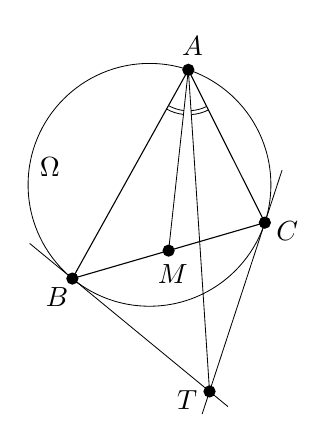
\begin{tikzpicture}[x=0.35cm,y=0.35cm]
			%\clip (-4.66,-6.97) rectangle (5.17,6.77);
			\draw [line width=0.3] (-0.186,1.372) circle (4.405);
			\coordinate (A) at (1.224,5.545);
			\coordinate (B) at (-2.984,-2.03);
			\coordinate (C) at (4,0);
			\coordinate (M) at (0.508,-1.015);
			\coordinate (T) at (1.993,-6.125);
			\draw (A) to (B) to (C) to cycle;
			\draw [line width=0.3] (M) to (A) to (T);
			\draw [line width=0.3,shorten <=-2em,shorten >=-2ex] (B) to (T);
			\draw [line width=0.3,shorten <=-2em,shorten >=-2ex] (C) to (T);
			\draw [line width=0.3,shift={(A)}] (240.945:0.57cm) arc (240.945:263.77:0.57cm);
			\draw [line width=0.3,shift={(A)}] (240.945:0.52cm) arc (240.945:263.77:0.52cm);
			\draw [line width=0.3,shift={(A)}] (273.77:0.57cm) arc (273.77:296.595:0.57cm);
			\draw [line width=0.3,shift={(A)}] (273.77:0.52cm) arc (273.77:296.595:0.52cm);
			\draw [fill=black] (A) circle (2pt) node[shift={(80:2ex)}] {$A$};
			\draw [fill=black] (B) circle (2pt) node[shift={(230:2ex)}] {$B$};
			\draw [fill=black] (C) circle (2pt) node[shift={(-20:2ex)}] {$C$};
			\draw [fill=black] (M) circle (2pt) node[shift={(280:2ex)}] {$M$};
			\draw [fill=black] (T) circle (2pt) node[shift={(200:2ex)}] {$T$};
			\node at (-3.8,2) {$\Omega$};
		\end{tikzpicture} & & 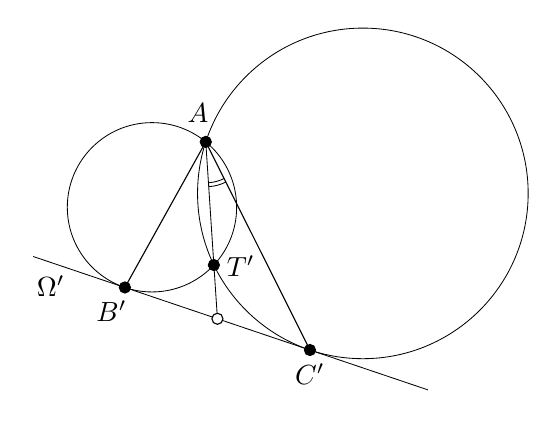
\begin{tikzpicture}[x=0.35cm,y=0.35cm]
			%\clip (-4.96,-3.45) rectangle (12.98,9.74);
			\draw [line width=0.3] (-0.728,3.173) circle (3.072);
			\draw [line width=0.3] (6.924,3.677) circle (5.998);
			\coordinate (A) at (1.224,5.545);
			\coordinate (B) at (-1.711,0.263);
			\coordinate (C) at (5.004,-2.006);
			\coordinate (M) at (1.647,-0.872);
			\coordinate (T) at (1.518,1.077);
			\draw (B) to (A) to (C);
			\draw [line width=0.3,shorten <=-3.5em,shorten >=-4.5em] (B) to (C);
			\draw [line width=0.3] (M) to (A) to (T);
			\draw [line width=0.3,shift={(A)}] (273.77:0.52cm) arc (273.77:296.595:0.52cm);
			\draw [line width=0.3,shift={(A)}] (273.77:0.57cm) arc (273.77:296.595:0.57cm);
			\draw [fill=black] (A) circle (2pt) node[shift={(105:2.5ex)}] {$A$};
			\draw [fill=black] (B) circle (2pt) node[shift={(240:2.25ex)}] {$B'$};
			\draw [fill=black] (C) circle (2pt) node[shift={(270:2ex)}] {$C'$};
			\draw [fill=white] (M) circle (2pt);
			\draw [fill=black] (T) circle (2pt) node[shift={(-2:2.25ex)}] {$T'$};
			\node at (-4.4,0.3) {$\Omega'$};
		\end{tikzpicture} & \\
		& vor Inversion & & nach Inversion &
	\end{tabularx}
\end{figure}
\begin{proof}
	Wir invertieren an $A$; die Bildpunkte von $B$, $C$ und $T$ bezeichnen wir mit $B'$, $C'$ und $T'$. Der Kreis $\Omega$ durch $A$, $B$ und $C$ wird auf die Gerade $B'C'$ abgebildet. Die Tangenten an $\Omega$ in $B$ und $C$ werden auf Kreise durch $A$ abgebildet, die das Bild von $\Omega$, also die Gerade $B'C'$, berühren. Schließlich ist $T'$ der von $A$ verschiedene Schnittpunkt dieser beiden Kreise. Insbesondere muss $AT'$ die Potenzgerade der beiden Kreise sein. Folglich führt $AT'$ durch den Mittelpunkt ihrer gemeinsamen Tangente $\overline{B'C'}$, also ist $AT'$ die Seitenhalbierende von $\overline{B'C'}$. Nach einer bekannten Eigenschaft der Inversion sind $ABC$ und $AB'C'$ gegensinnig ähnlich sind. Weil die Seitenhalbierenden $AM$ und  $AT'$ einander entsprechen, erhalten wir $\winkel MAC=\winkel B'AT'$. Andererseits erhält Inversion an $A$ Winkel mit Scheitelpunkt $A$. Also gilt $\winkel BAT=\winkel B'AT'$. Es folgt $\winkel BAT=\winkel MAC$. Damit ist gezeigt, dass~$T$ auf dem Symmedian durch~$A$ liegt.
\end{proof}

Im Kapitel \emph{Projektive Geometrie} im Heft für Klasse~11 habt ihr gelernt, dass zwei Punktepaare $(A,B)$ und $(C,D)$ auf einem Kreis $\Omega$ genau dann harmonisch liegen, wenn der Pol von $AB$ auf $CD$ liegt. Aber der Pol von $AB$ ist genau der Schnittpunkt der Tangenten an $\Omega$ in $A$ und $B$. Wir erhalten also auch, dass $(A,B)$ und $(C,D)$ genau dann harmonische Punktepaare sind, wenn $D$ auf dem Symmedian von $ABC$ durch $C$ liegt.

\subsection*{Tipps zu den Beispielaufgaben}
\textbf{Tipps zu Aufgabe~\ref{aufgabe:MEMO2014}.} Was weißt du über die Gerade $AD$ sowie die In- und Ankreisberührpunkte mit $\overline{BC}$? Fällt dir in deiner Skizze etwas auf?

Findest du die Winkel $\winkel BLD$ und $\winkel DLC$ an anderer Stelle in deiner Skizze wieder? Kannst du damit zeigen, dass $BNCL$ ein Sehnenviereck ist?

\textbf{Tipps zu Aufgabe~\ref{aufgabe:PolenMO2019}.} Zeige, dass die Behauptung äquivalent dazu ist, dass $AR$ der Symmedian durch $A$ im Dreieck $ABC$ ist. Nach dem Symmedian-Lemma verläuft dieser Symmedian auch durch den Schnittpunkt $T$ der Tangenten an $\Omega$ in $B$ und $C$. Zeichne $T$ in deine Skizze ein. Was fällt dir dabei auf?

Die Aussage ist nun äquivalent dazu, dass sich $AT$, $DQ$ und $EP$ in einem Punkt schneiden. Formuliere diese Aussage mithilfe des Satzes von Desargues um. Um die neue Aussage zu zeigen, betrachte zum Beispiel die Streckung mit Zentrum $P$, die $\omega_E$ auf $\Omega$ abbildet.